\subsection{The architecture}

When designing the architecture of our network, we took inspiration from LeNet \cite{lenet5}. The model was designed to classify grey-scale images of handwritten digits, where the main indicators of each class are its morphological features. Images in our work are very similar and the difference between each class also relies on the object's morphological features, such as shape, density, etc. 

% prepisat este
The dimensions of the input data to the LeNet network are not consistent with the size of our data. As for this, the topology of the LeNet5 network needed some modifications, to be able to fit our input data. Some changes were made regarding the number of layers and the dimensions of kernels in convolutional layers. 

The topology of network is demonstrated in the Figure \ref{img:arch0} and consists of following layers: 

\begin{enumerate}
    \item \textbf{Layer C1} \\
    The first convolution layer consists of 6 kernels of size 5x5. The convolution operation is performed using a stride of 1 with zero padding on the image. The input to the layer is the grey-scale image of 50x50x1 and the output feature maps are of size 46x46, which makes the output volume 46x46x6. The layer has a total of 156 learnable parameters, including 150 weights and 6 biases. 
    
    \item \textbf{Layer S2} \\
    Subsampling layer that uses average pooling with a kernel of 2x2 size and stride of 2. The input volume to the layer is 46x46x6, and the pooling layer reduces the spatial size by a factor of 2, while the depth stays the same. This results in an output volume of 23x23x6.
    
    \item \textbf{Layer C3} \\
    The second convolution layer with 16 kernels of size 4x4, moving with a stride of 1 and zero padding on the input data. The output consists of 16 feature maps of size 20x20. The layer introduces 96 weights and 1 bias per filter, which is a total of 1552 learnable parameters.
    
    \item \textbf{Layer S4} \\
    The structure of the subsampling layer is the same as the layer S2. The input to the layer is a volume of 20x20x16 which makes the output 10x10x16.
    
    \item \textbf{Layer C5} \\
    The third convolution layer with 32 kernels of size 5x5. Again moving with a stride of 1 and zero padding. The layer outputs the volume 6x6x32. It has a total of 12 832 learnable parameters, with 400 weights and 1 bias per filter. 
    
    \item \textbf{Layer S6} \\
    The last subsampling layer, with the same structure as the previous ones. The layer receives the input volume of 6x6x32 and outputs 32 feature maps of size 3x3.
    
    \item \textbf{Layer C7} \\
    The last convolution layer consists of 120 3x3 convolution kernels, moving with a stride of 1 and zero padding on the input data. As the dimensions of the input data are the same as the convolution kernel, the output is one dimensional tensor with a length of 120. The layer has 289 parameters per filter, which results in a total of 34 680 learnable parameters. 
    
    \item \textbf{Layer F8} \\
    The first fully connected layer contains 84 neurons. The input to the layer is a tensor with a length of 120, or we can also imagine it as 120 neurons. Each neuron from the input is connected to each neuron in the layer. This makes a total of 10 080 connections, where each connection introduces one learnable weight. Each neuron in the layer also contains one bias value. This gives a total of 10 164 learnable parameters.
    
    \item \textbf{Layer F9} \\
    The second fully connected layer where the number of neurons is the number of classes. In the case of LeNet5, it was 10 but in our case, it's 6 neurons. Connecting with the previous layer with 84 neurons creates 504 weights and 6 biases, for a total of 510 learnable parameters. 
\end{enumerate}

The network is made up of 9 layers and has a total of 59 894 learnable parameters. It is standard practice for the topology to consist of alternating convolutional and pooling layers, followed by fully-connected layers at the end. 

Important to mention, that after each convolutional and fully-connected layer, non-linear activation is applied to the data. The specific choice of activation function is not mentioned here as it will be a hyperparameter determined by validation of the network. 


\begin{figure}[h]
    \centering
    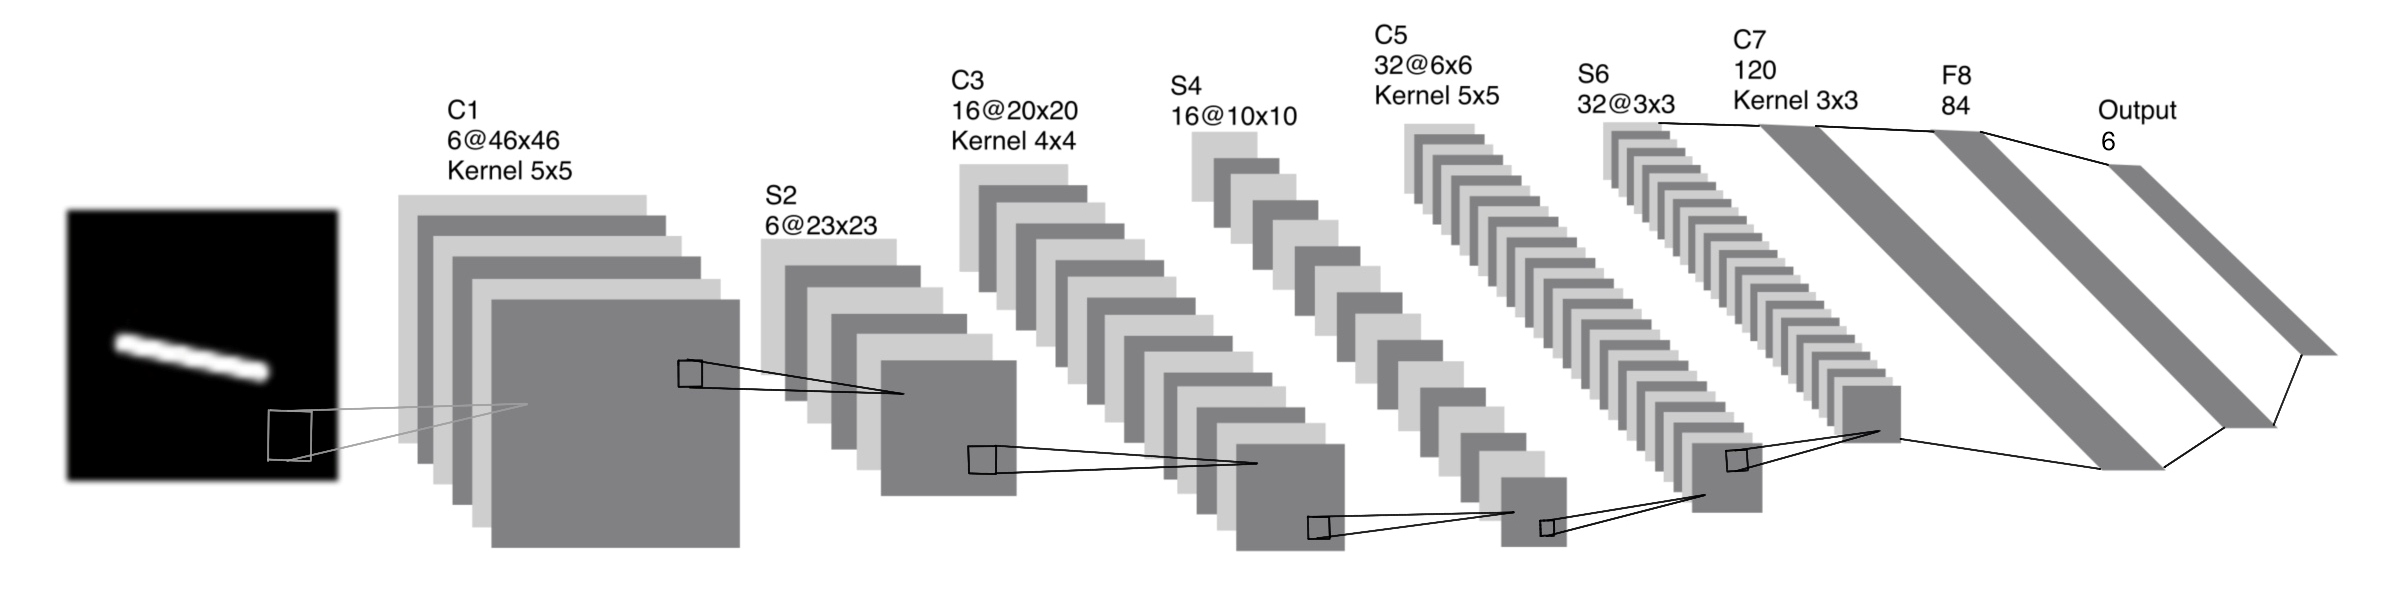
\includegraphics[width=\textwidth]{images/architectureCNN2.png}
    \caption[The proposed architecture of the neural network]
    {The proposed architecture of the neural network. 
    For each convolutional layer (denoted as “C”) the information about the kernel and size of output feature maps is defined (N@MxM, where N is the number of filters used and MxM is the spatial size of the feature maps). 
    Subsampling layers ("S") always operate with a 2x2 kernel and reduce only the spatial size of the feature maps. The output information is defined in the same way as with convolutional layers. 
    The last two layers of the network are fully connected ("F") and specify the number of neurons in the layer. The last fully-connected layer is denoted as the output layer.}
    \label{img:arch0}
\end{figure}
